\documentclass[12pt]{article}
\usepackage{tikz}
\usepackage{pgfplots}
\usepackage{bm}
\usepackage[margin=1in]{geometry}
\usepackage{hyperref}
\usepackage{amsmath}
\usepackage{amssymb}
\hypersetup{colorlinks=true, linkcolor=blue, filecolor=blue, citecolor = black, urlcolor=cyan}
\pgfmathsetseed{1234}
\usetikzlibrary{fit,positioning,calc,shapes,backgrounds}
\usetikzlibrary{shapes.geometric, arrows}
\tikzset{>=latex}
\usepackage{tikz-feynman}
\pgfkeys{/tikzfeynman/warn luatex=false}
\usepgfplotslibrary{groupplots}
% \includeonlyframes{current}
\usepackage{umnparticles}
\usepackage{listings}
\usepackage{graphicx}



\definecolor{codegreen}{rgb}{0,0.6,0}
\definecolor{codegray}{rgb}{0.5,0.5,0.5}
\definecolor{codepurple}{rgb}{0.58,0,0.82}
\definecolor{backcolour}{rgb}{0.95,0.95,0.92}
\lstdefinestyle{mystyle}{
  backgroundcolor=\color{backcolour},   
  commentstyle=\color{codegreen},
  keywordstyle=\color{magenta},
  numberstyle=\tiny\color{codegray},
  stringstyle=\color{codepurple},
  basicstyle=\ttfamily\footnotesize,
  breakatwhitespace=false,         
  breaklines=true,                 
  captionpos=b,                    
  keepspaces=true,                 
  numbers=left,                    
  numbersep=5pt,                  
  showspaces=false,                
  showstringspaces=false,
  showtabs=false,                  
  tabsize=2
}
\lstset{style=mystyle}


\title{Update On Model Selection for the Single-Stop Analysis}
\date{\today}
\author{Nadja Strobbe \and Devin Mahon \and Charlie Kapsiak \and Shardul Rao \and Seth Bendigo}


\graphicspath{{./figures}}
\newcommand{\commonfiles}[1]{../common/#1}
\usepackage[mode=buildnew]{standalone}


\begin{document}

\maketitle{}

\section{Background}

Earlier this month, we gave a \href{https://indico.cern.ch/event/1459336/\#9-statistical-inquiry-on-non-p}{talk} to the statistics committee  on our background estimation procedure for a RPV-SUSY search. 

\begin{center}
  % \graphiccite{figures/xsec.png}{0.5}{rasmussen_gaussian_2006}\hspace{1em}
  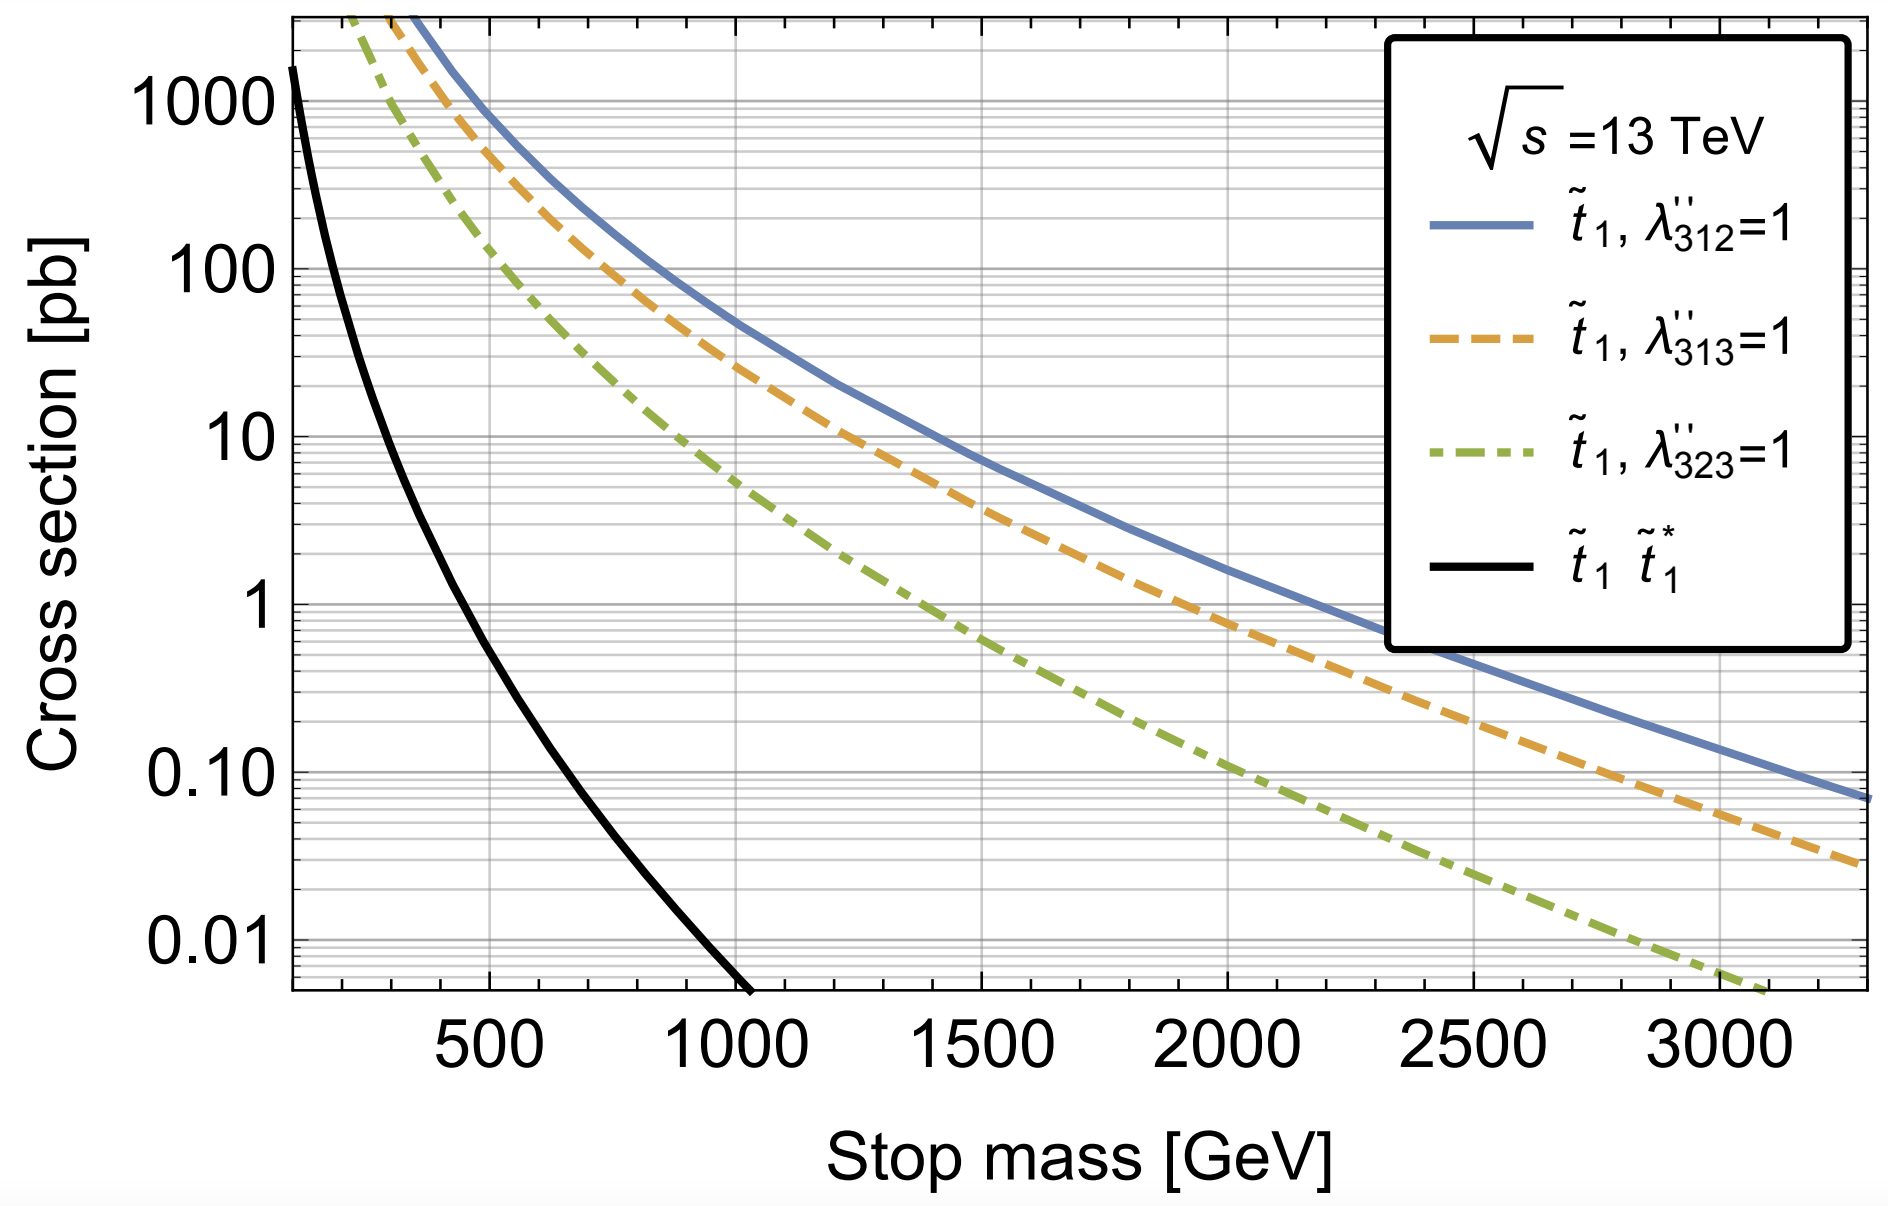
\includegraphics[width=0.5\textwidth]{figures/xsec.png}
  \hspace{1cm}
  \scalebox{1}{\includestandalone{\commonfiles{general/single_stop}}}
\end{center}

The core search strategy involves the simulatenous reconstruction of both the $\chargino{}$ and the \stopq{}, and doing a 2 dimensional bump hunt in the cases where the resonances are at least partially un-correlated.


The technique we have chosen to use is Gaussian process regression.
We have found that this technique can produce good estimations of the background, but it was less clear to us how to handle potential systematics from the modeling itself. 


\section{Key Question}
As a kernel machine, the key choice for GPR is the choice of kernel, which parametrizes the correlations between points.
The choice of kernel involves both it function form and its hyperparameters.
Gaussian process regression furnishes and inherent uncertainty.
However, to form the regression in to a valid statistical procedure, we need to determine to what extent the model selection affects the posterior regression.
\begin{enumerate}
\item The goal is to determine whether a systematic for hyperparameter optimization is needed, or if the model itself has uncertainties that cover variations.
\end{enumerate}

\textbf{The suggestion from the committee was to inspect the posterior predictive distribution, and to see how well it fits the data.
}

Specifically, the output of the GPR is a distribution over ``latent'' functions,
\begin{equation}
  f \sim \mathcal{GP} \left( m(x), k(x,x') \right) 
\end{equation}
If we are interested in the observed values, rather than the latent function $f$, then we need to not the distributions over the observed outputs y$^{*}$.
\begin{equation}
  P(y^{*}) = \int P(y^{*} | f^{*}) P(f^{*}| x^{*},X,y,\theta)
\end{equation}
where $P(y^{*} | f^{*}) $ is the likelihood, and $x^{*},X,y,\theta$ are the test points, training points, training inputs, and hyperparamets, respectively. 

Since the true likelihood is Poisson, we use simulation to construct the posterior predictive distribution.
Given our posterior process $MVN$, we simulate distribution $P(y^{*})$.

To we estimate the uncerainty on the posterior distributions (for the purpose of generating pull plots), we use the variance of the posterior predictive distribution. 

{\bfseries The goal is to determine if this posterior predictive distribution accurately models the data.}

\section{Results of Study}

We find that for most of the plane, the posterior predictive uncertainty is dominated by the Poisson likleihood, rather than the Gaussian uncertainty on the latent function.
At the edges of the plane, the lower values and the fewer points to ``smooth'' over means that the GPR uncertainty becomes dominant.
However, for the remainder of the plane, including all areas where we have signal points, the relative uncerainty of the GPR is quite small, so the variance of the Poisson likelihood is dominant.


Our conclusion is that 




\end{document}

% Local Variables:
% eval: (progn (setq process-environment (copy-sequence process-environment))
% (let* ( (basedir (file-name-directory (directory-file-name (file-name-directory (buffer-file-name)))))
% (texmfpath (file-name-concat  basedir "texmf"))
% )
% (setq-local TeX-style-path (append TeX-style-path  (directory-files-recursively texmfpath "auto" t)))
% (setq-local reftex-bib-path (list basedir))
% (setenv "TEXMFHOME" texmfpath )
% (setenv "BIBINPUTS" basedir ))
% )
% End:
